\documentclass[tikz,border=2pt,11pt]{standalone}
\usetikzlibrary{arrows.meta}
\usetikzlibrary{calc}
\usetikzlibrary{positioning}
\usepackage{amsmath}
\usepackage{amssymb}
\usepackage{tikz}
\def\UrlBreaks{\do\/\do-\do.\do_}
\newcommand{\C}{\mathbb C}
\newcommand{\Z}{\mathbb Z}
\newcommand{\N}{\mathbb N}
\newcommand{\Q}{\mathbb Q}
\newcommand{\R}{\mathbb R}
\newcommand{\K}{\mathcal K}
\DeclareMathOperator{\KK}{KK}
\DeclareMathOperator{\KX}{KX}
\DeclareMathOperator{\id}{id}
\DeclareMathOperator{\prop}{prop}
\DeclareMathOperator{\supp}{supp}
\DeclareMathOperator{\Ad}{Ad}
\DeclareMathOperator{\SL}{SL}
\begin{document}
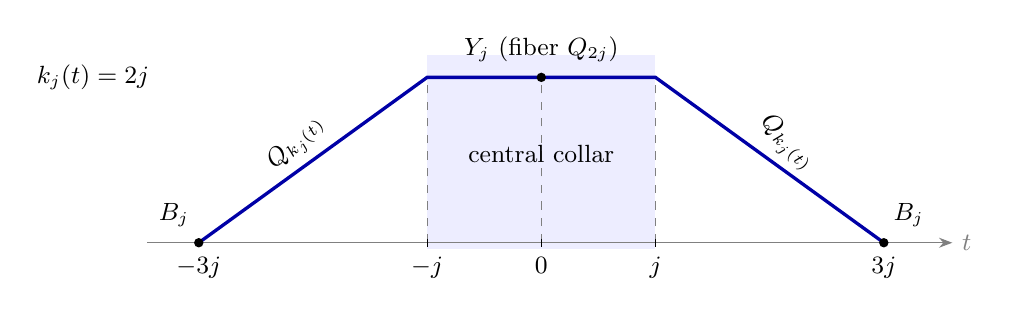
\begin{tikzpicture}[x=1.45cm,y=1.05cm,>=Stealth,font=\small]
 \fill[blue!7] (-1,-0.08) rectangle (1,2.27);
 \draw[->,gray] (-3.45,0)--(3.6,0) node[right] {$t$};
 \draw[very thick,blue!65!black] (-3,0)--(-1,2)--(1,2)--(3,0);
 \draw[dashed,gray] (-1,0)--(-1,2);
 \draw[dashed,gray] (1,0)--(1,2);
 \draw[dashed,gray] (0,0)--(0,2);
 \foreach \x/\lab in {-3/{-3j},-1/{-j},0/{0},1/{j},3/{3j}}{
  \draw (\x,0.05)--(\x,-0.05);
  \node[below] at (\x,-0.06) {$\lab$};
 }
 \fill (-3,0) circle (1.7pt);
 \fill (3,0) circle (1.7pt);
 \fill (0,2) circle (1.7pt);
 \node[above left] at (-3,0.08) {$B_j$};
 \node[above right] at (3,0.08) {$B_j$};
 \node[above] at (0,2.07) {$Y_j$ (fiber $Q_{2j}$)};
 \node at (0,1.08) {central collar};
 \node[rotate=45,above] at (-2,1) {$Q_{k_j(t)}$};
 \node[rotate=-45,above] at (2,1) {$Q_{k_j(t)}$};
 \node[anchor=east] at (-3.35,2) {$k_j(t)=2j$};
\end{tikzpicture}
\end{document}
